

\documentclass{standalone}

\usepackage{tikz}
\usepackage{pgfplots}
\usepackage[cmex10]{amsmath}
\usepackage{amsfonts}
 \pgfplotsset{compat=1.12}
%\usepgfplotslibrary{polar}

\begin{document}

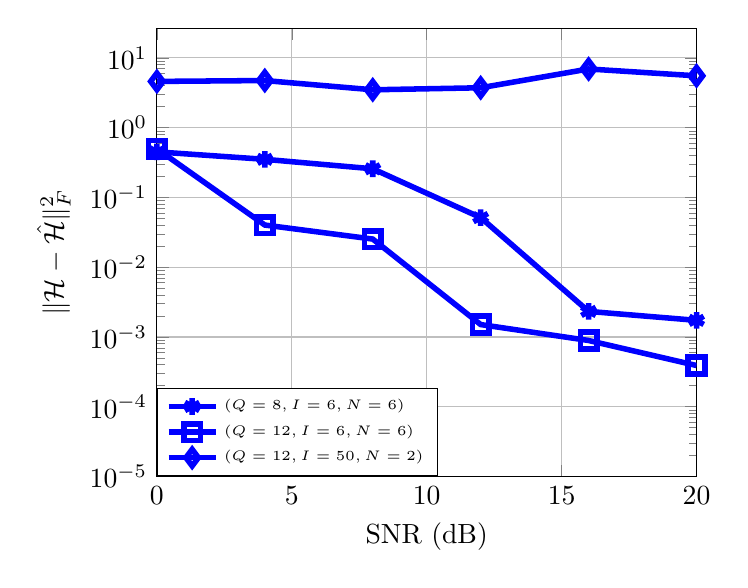
\begin{tikzpicture}

  \begin{axis}[%
    ymode = log,
%scale only axis,
%separate axis lines,
%every outer x axis line/.append style={black},
%every x tick label/.append style={font=\color{black}},
xmin=0,
xmax=20,
xlabel={SNR (dB)},
%xmajorgrids,
%every outer y axis line/.append style={black},
%every y tick label/.append style={font=\color{black}},
ylabel={ $\|\mathcal{H} - \hat{\mathcal{H}}\|^2_F$},
% title = Channel frequency response between $\mathbf{H}(2,1)$,
ymin = 0.00001,
grid,
%axis background/.style={fill=white},
legend style={at={(0,0)},anchor=south west,legend cell align=left,align=left,draw=black,font=\fontsize{4}{5}\selectfont}
]

%%%%%%%%%%%%%%%%%%%%%%%%% M=8 %%%%%%%%%%%%%%%%%%%%%%%%%%%%%%%%%%%%%%%%%%%%%%%%%


\addplot [color=blue,solid,mark=asterisk,mark options={solid},line width=2pt,mark size=3pt]
  table[row sep=crcr]{%
0 0.44937 \\
4 0.3513 \\
8 0.25693 \\
12 0.05133 \\
16 0.0023251 \\
20 0.001731 \\
};
\addlegendentry{$(Q=8,I=6,N=6)$}; 

\addplot [color=blue,solid,mark=square,mark options={solid},line width=2pt,mark size=3pt]
  table[row sep=crcr]{%
0 0.49713 \\
4 0.040181 \\
8 0.025289 \\
12 0.0015062 \\
16 0.0008905 \\
20 0.0003901 \\
};
\addlegendentry{$(Q=12,I=6,N=6)$}; 


\addplot [color=blue,solid,mark=diamond,mark options={solid},line width=2pt,mark size=3pt]
  table[row sep=crcr]{%
0 4.5925 \\
4 4.7258 \\
8 3.4832 \\
12 3.7243 \\
16 6.92 \\
20 5.5225 \\
};
\addlegendentry{$(Q=12,I=50,N=2)$}; 





\end{axis}
\end{tikzpicture}%
\end{document}


%%% Local Variables:
%%% mode: latex
%%% TeX-master: t
%%% End:
